\documentclass[11pt,letterpaper]{article}

\newenvironment{proof}{\noindent{\bf Proof:}}{\qed\bigskip}

\newtheorem{theorem}{Theorem}
\newtheorem{corollary}{Corollary}
\newtheorem{lemma}{Lemma} 
\newtheorem{claim}{Claim}
\newtheorem{fact}{Fact}
\newtheorem{definition}{Definition}
\newtheorem{assumption}{Assumption}
\newtheorem{observation}{Observation}
\newtheorem{example}{Example}
\newcommand{\qed}{\rule{7pt}{7pt}}

\newcommand{\solution}[4]{
\thispagestyle{plain} 
\newpage
\setcounter{page}{1}
\noindent
\begin{center}
\framebox{ \vbox{
\vspace{4mm}
\vspace{0.2in} 
{\centering \large\mbox{#3}}\\
\vspace{0.1in}
{#1 \hfill {Date: #2}}
}}
\end{center}
\markright{#1}
}

\newenvironment{algorithm}
{\begin{center}
\begin{tabular}{|l|}
\hline
\begin{minipage}{1in}
\begin{tabbing}
\quad\=\qquad\=\qquad\=\qquad\=\qquad\=\qquad\=\qquad\=\kill}
{\end{tabbing}
\end{minipage} \\
\hline
\end{tabular}
\end{center}}

\def\Comment#1{\textsf{\textsl{$\langle\!\langle$#1\/$\rangle\!\rangle$}}}


\usepackage{graphicx}
\usepackage{float}
\usepackage{multicol}
\usepackage{balance}
\usepackage{multicol}
\usepackage{multirow}
\usepackage{epstopdf}
\usepackage{epsfig}
\usepackage{makeidx}
\usepackage{bm}
\usepackage{pbox}
\usepackage{pdflscape}
\usepackage{url}
\usepackage{framed}
\usepackage{mathtools}
\usepackage{adjustbox}
\usepackage{amsmath}
\usepackage{hyperref}
\usepackage{subcaption}
\usepackage{cite}
\usepackage{amsfonts}

\usepackage{graphicx, amssymb, amsmath, listings, float, mathtools}
\usepackage{color, url}
\lstset{language = Python}
\lstset{breaklines}
\lstset{extendedchars=false}

\oddsidemargin 0in
\evensidemargin 0in
\textwidth 6.5in
\topmargin -0.6in
\textheight 9.0in

\begin{document}

\solution{\large Jifu Zhao}{\large 02/18/2018}{\bf \Large STAT 578  \hspace{0.5cm} 
		Spring 2018 \hspace{0.5cm} Homework 1}


\section*{(a)}

\begin{table}[htb]
 \caption{Summary of Cross Validation} \label{result}
 \vspace{0.1in}
\begin{center}
  \begin{tabular}{  c  c  c}
    \hline
    RMSE/Model        & Linear Regression        & KNN      \\ \hline
    CV 1                     & 1.13332                           & 1.15368 \\ \hline
    CV 2                    & 1.11352                            & 1.13066 \\ \hline
    CV 3                    & 1.09645                           & 1.11158 \\ \hline
    CV 4                    & 1.09598                           & 1.11329 \\ \hline
    CV 5                    & 1.09997                           & 1.11868  \\ \hline
    Mean                   & 1.10785                           &  1.12558 \\ \hline 
    Std                      & 0.01424                           &  0.01556 \\ \hline 
  \end{tabular}
\end{center}
\end{table}

\section*{(b)}


\begin{figure}[H]
\centering
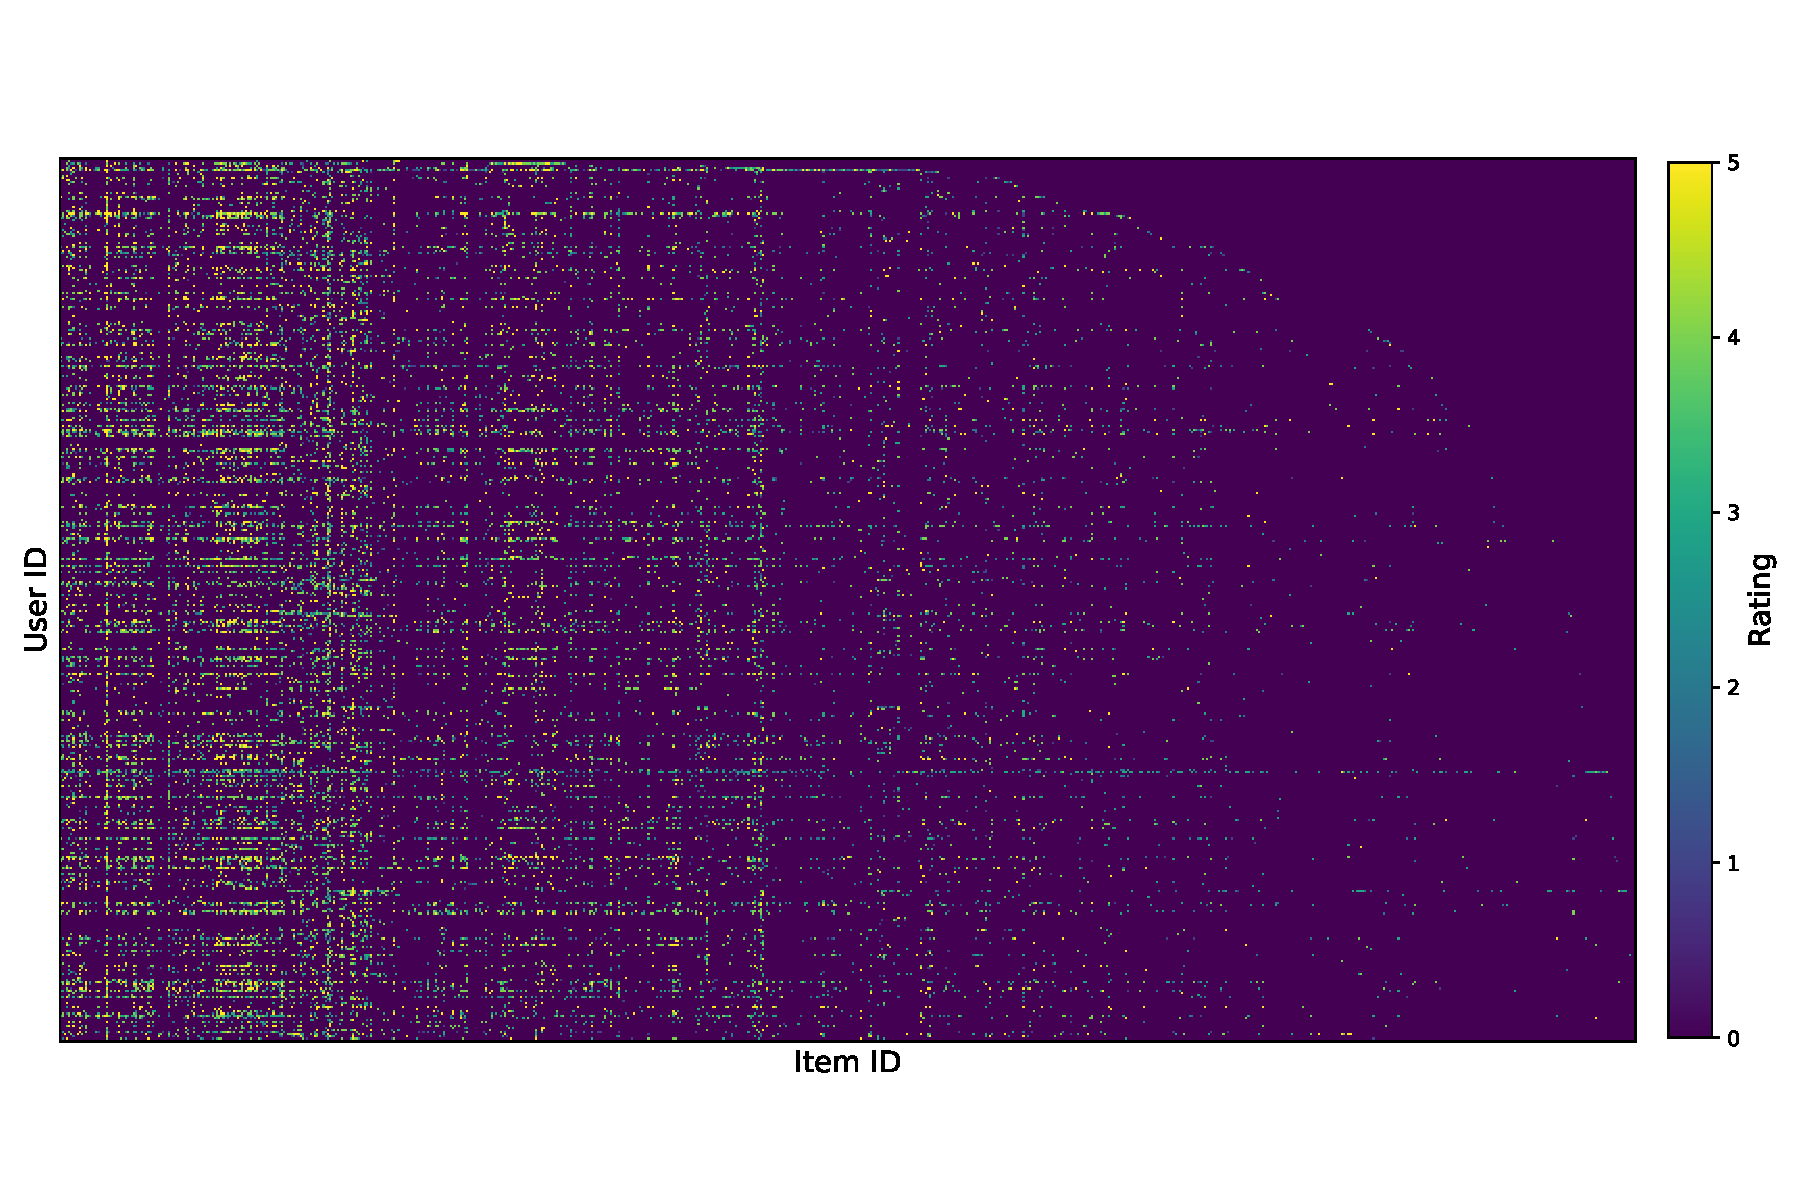
\includegraphics[width=1.0\textwidth]{./figures/utility.pdf}
\caption{\label{fig:utility} User-item utility matrix}
\end{figure}

\begin{figure}[htbp]
\centering
\begin{subfigure}[b]{0.5\linewidth}
  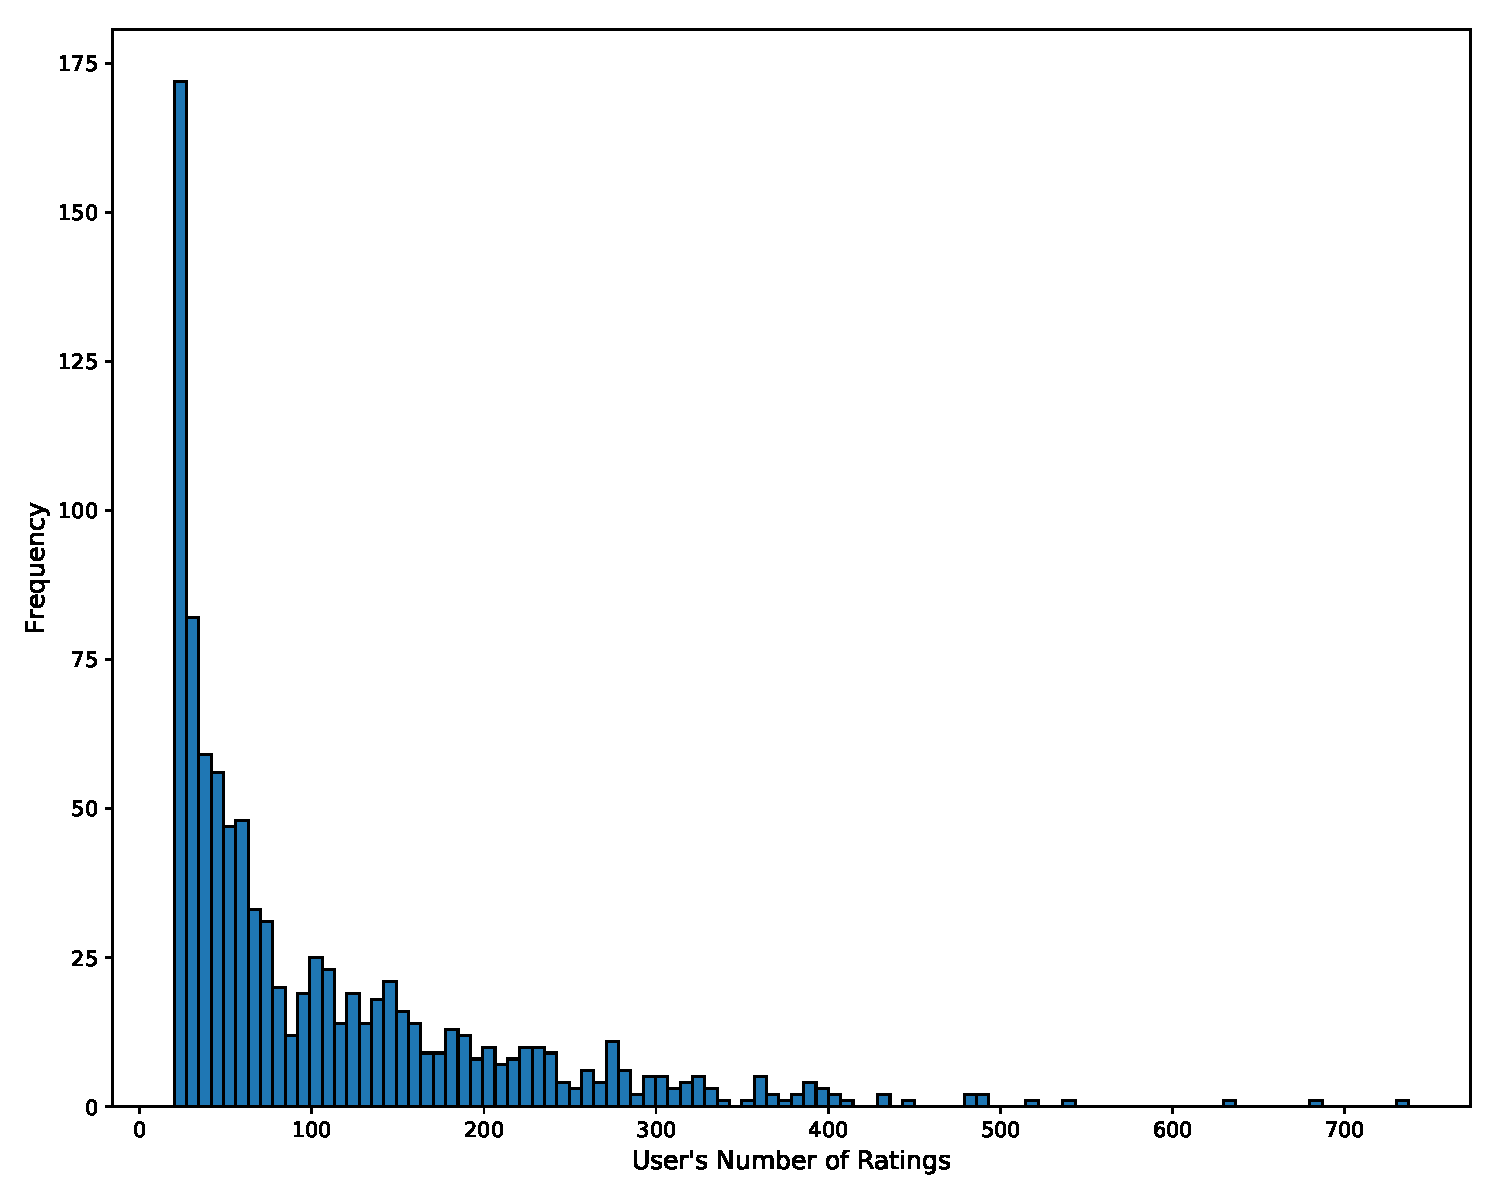
\includegraphics[width=1.00\textwidth]{./figures/user_frequency.pdf}
  \caption{Distribution of user's number of ratings}
   \label{ex_without_source}
\end{subfigure}%
\begin{subfigure}[b]{0.5\linewidth}
  \centering
  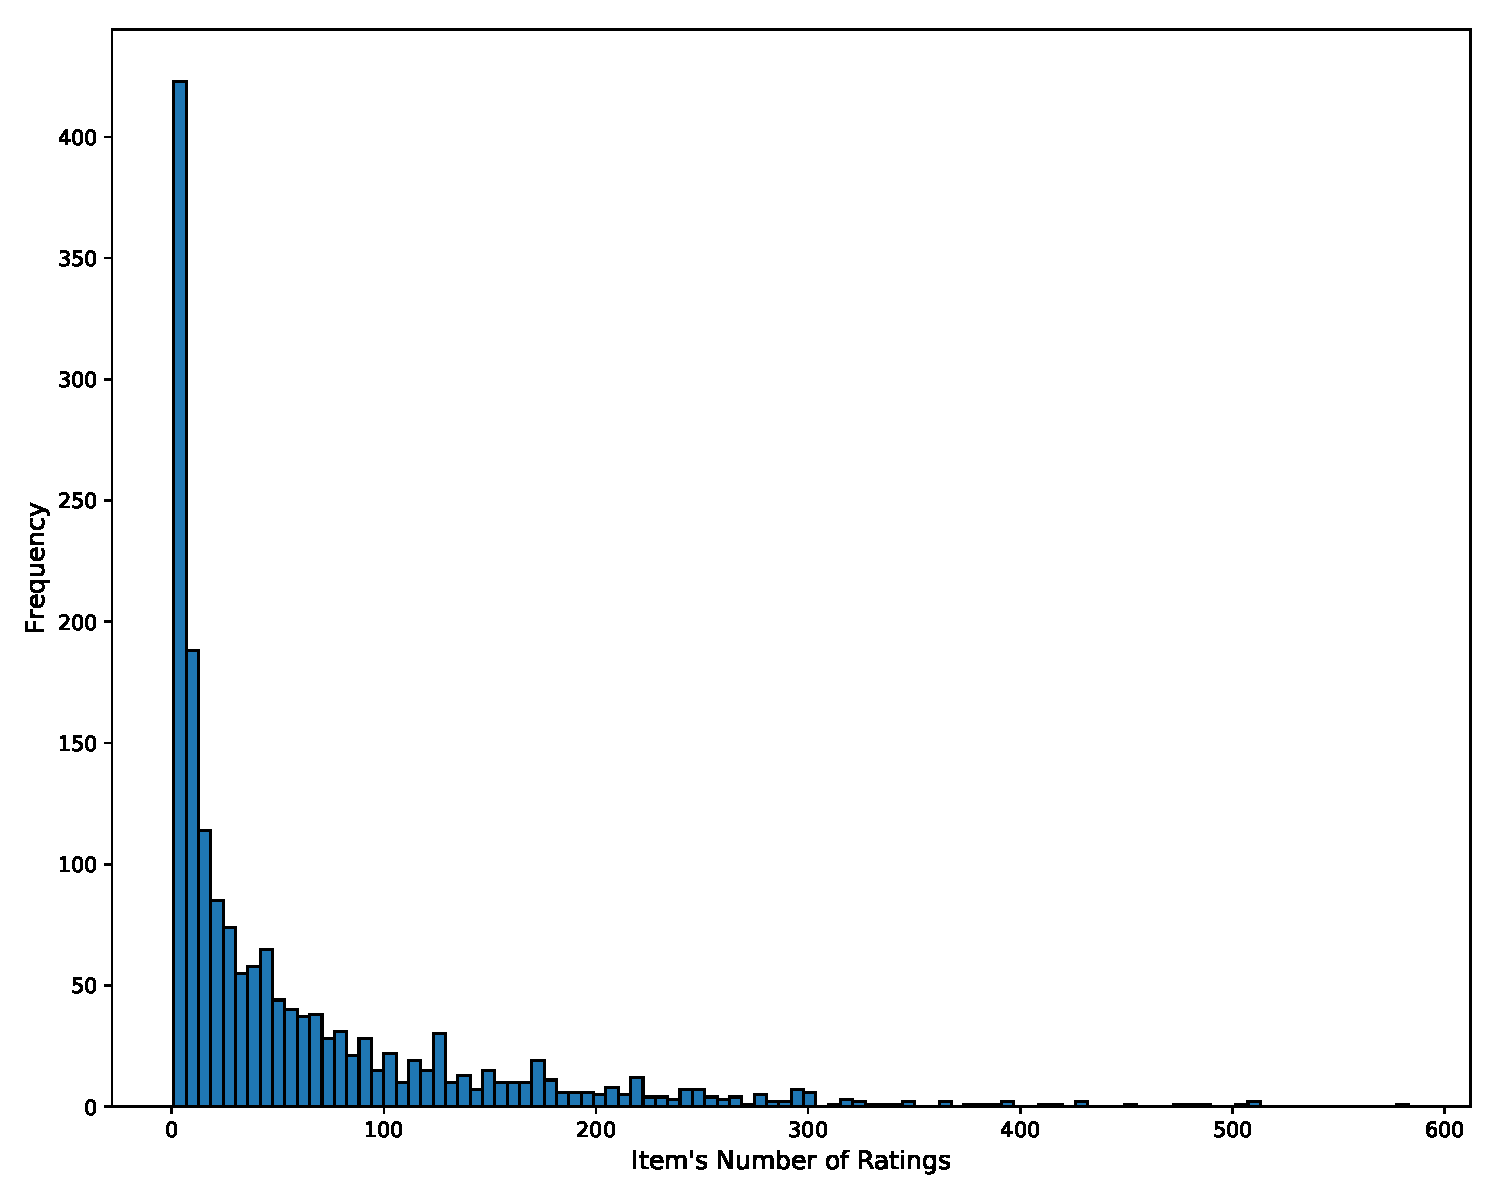
\includegraphics[width=1.00\textwidth]{./figures/item_frequency.pdf}
  \caption{Distribution of item's number of ratings}
  \label{ex_with_source}
\end{subfigure}%
\raggedright
\caption{Distribution of User's / Item's number of ratings}
\label{fig:source_injection}
\end{figure}


\begin{figure}[htbp]
\centering
\begin{subfigure}[b]{0.5\linewidth}
  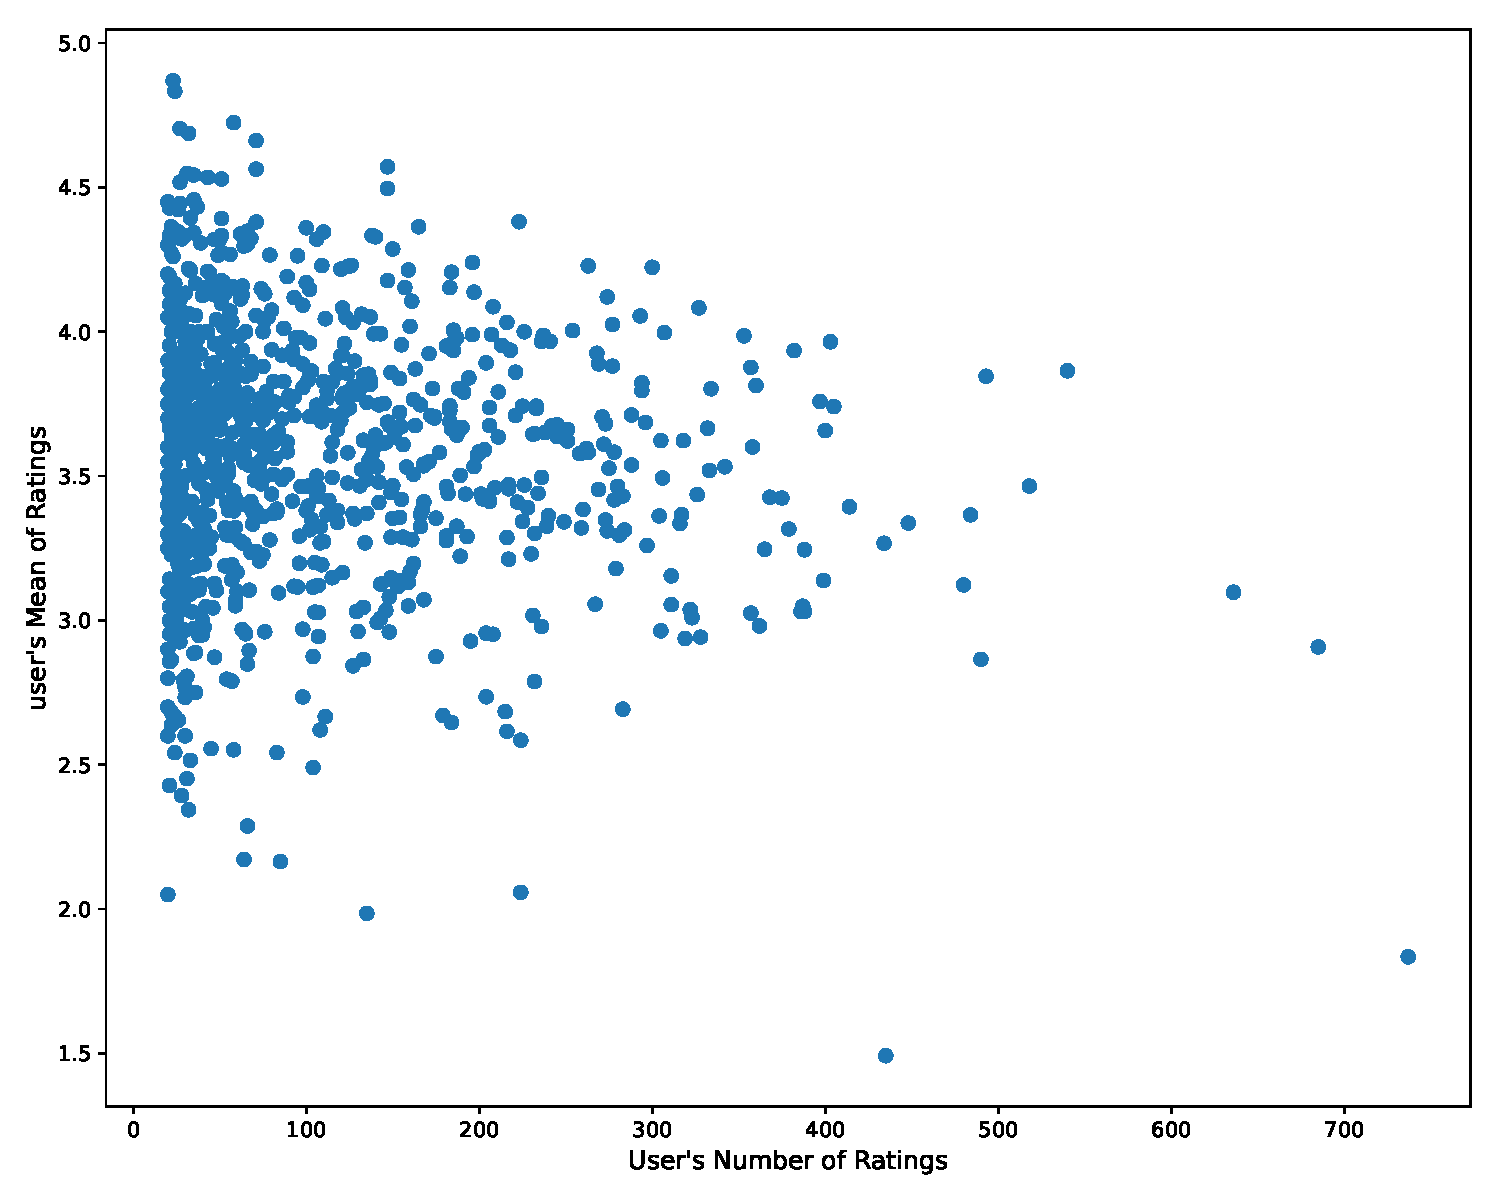
\includegraphics[width=1.00\textwidth]{./figures/user_mean_rating.pdf}
  \caption{User's mean rating vs. number of ratings}
   \label{ex_without_source}
\end{subfigure}%
\begin{subfigure}[b]{0.5\linewidth}
  \centering
  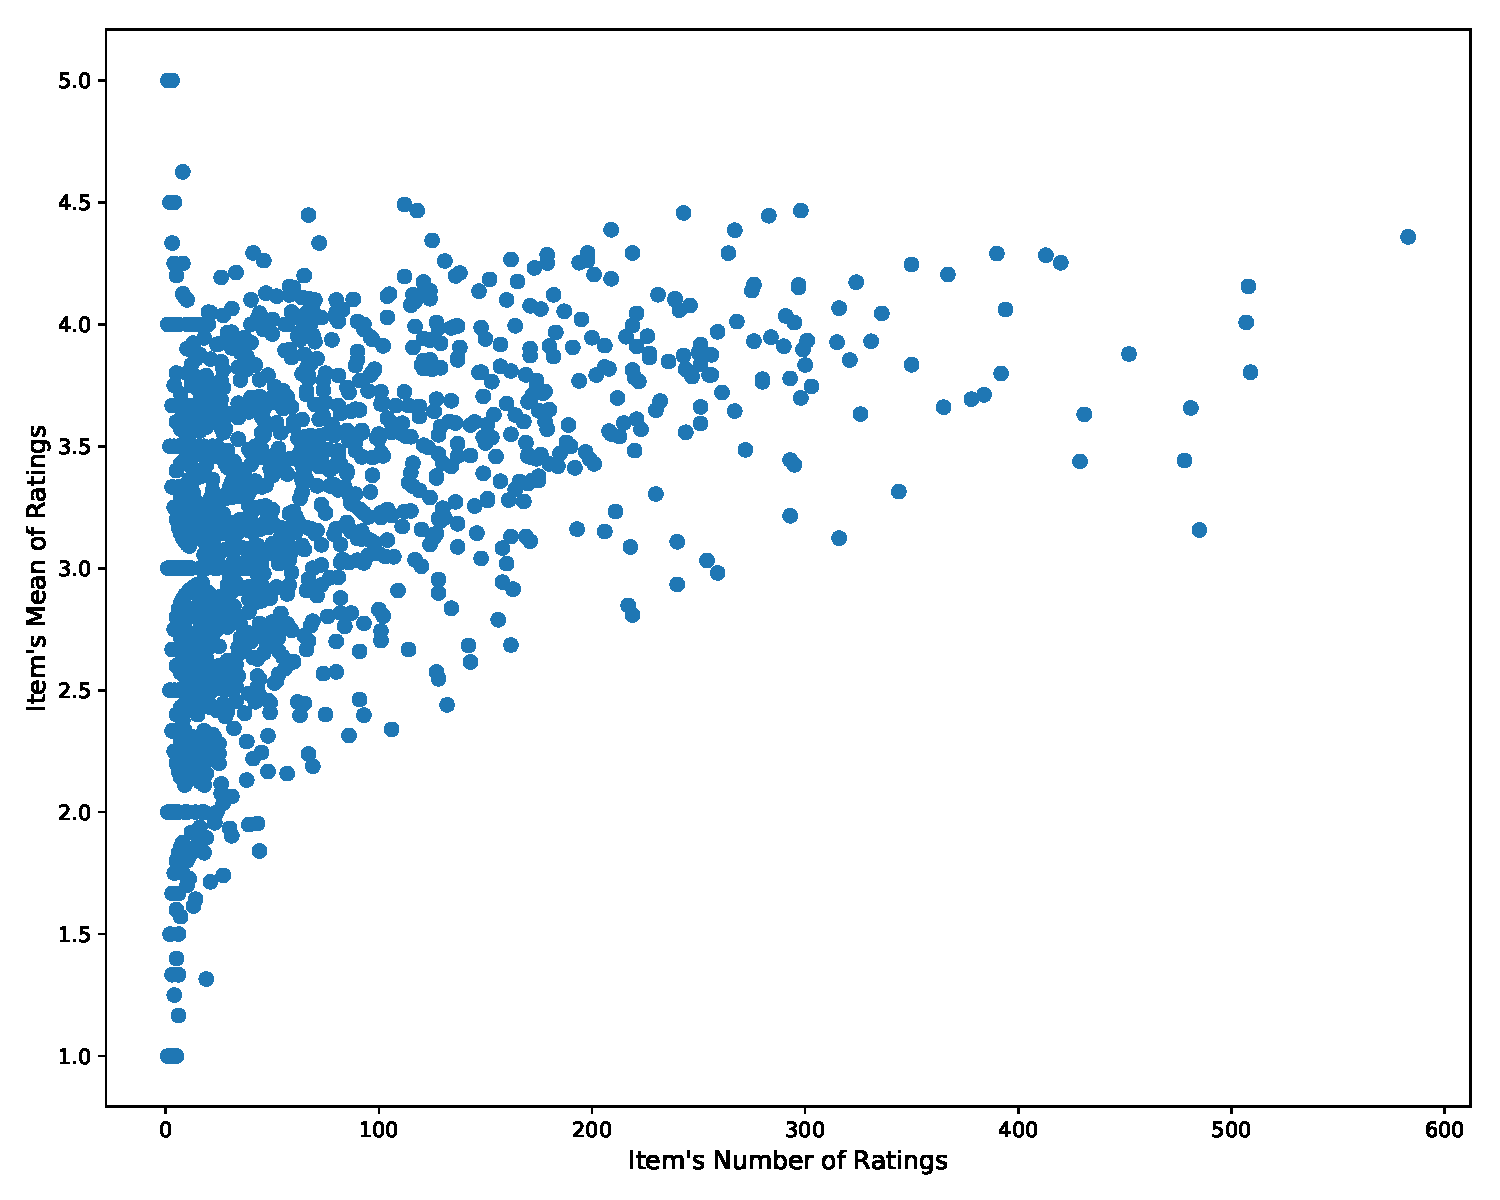
\includegraphics[width=1.00\textwidth]{./figures/item_mean_rating.pdf}
  \caption{Item's mean rating vs. number of ratings}
  \label{ex_with_source}
\end{subfigure}%
\raggedright
\caption{Mean ratings vs. number of ratings}
\label{fig:source_injection}
\end{figure}

\section*{(c)}

\begin{table}[htb]
 \caption{Summary of Cross Validation} \label{result}
 \vspace{0.1in}
\begin{center}
  \begin{tabular}{  c  c  c}
    \hline
    RMSE/Model        & Linear Regression        & KNN     \\ \hline
    CV 1                     & 1.10348                           & 1.12234 \\ \hline
    CV 2                    & 1.08674                           & 1.10264 \\ \hline
    CV 3                    & 1.07505                           & 1.08820 \\ \hline
    CV 4                    & 1.07059                           & 1.08572 \\ \hline
    CV 5                    & 1.07674                           & 1.09375 \\ \hline
    Mean                   & 1.08252                           &  1.09853 \\ \hline 
    Std                      &  0.01173                           &  0.01325 \\ \hline 
  \end{tabular}
\end{center}
\end{table}


\clearpage

%\bibliographystyle{plain}
%\bibliographystyle{unsrt}
%\bibliography{reference.bib}

\end{document}

